\subsubsection{Beispiel}
\label{bpr:algorithmus:beispiel}

\newcolumntype{M}[1]{>{\centering\arraybackslash}m{#1}}
\newcommand{\mc}[2]{\multicolumn{#1}{c}{#2}}

Am Beispiel \texttt{caabaccaabacaa} wird noch einmal die Funktionsweise des gesamten Algorithmus im Detail demonstriert. Das Beispiel dient der Übersichtlichkeit und Vergleichbarkeit zu anderen Algorithmen.
\begin{figure}[ht]
    {\centering\begin{minipage}{\textwidth}
        {\large \textsc{Schritt 1}} \hfill {\Large \textsc{Phase 1}}\par\medskip
        \resizebox{\textwidth}{!}{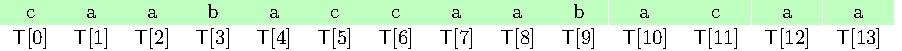
\includegraphics{kapitel/saca_algorithmen/bpr/algorithmus/beispiel/phase_1/step_01/t/image.pdf}}\par\bigskip
        \resizebox{\textwidth}{!}{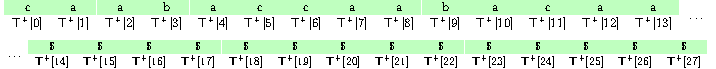
\includegraphics{kapitel/saca_algorithmen/bpr/algorithmus/beispiel/phase_1/step_01/tplus/image.pdf}}\\
    \end{minipage}}
    \caption[\bpr: Phase 1, Schritt 1]{\bpr: Phase 1, Schritt 1. Oben: Eingabetext \inputtext. Unten: Erweiterter Eingabetext \inputtextplus.}
    \label{bpr:p1s1}
\end{figure}
Der erste Schritt besteht lediglich daraus, die Eingabe aufzubereiten, indem \(n\) symbolische Sentinels an das Eingabewort angehängt werden. Dieses Vorgehen wird im Paper beschrieben, im Algorithmus allerdings aufgrund des linearen Speicherbedarfs nicht direkt umgesetzt. \par
\begin{figure}[ht]
    {\centering\begin{minipage}{\textwidth}
        {\large \textsc{Schritt 2}}\par\medskip
        \resizebox{\textwidth}{!}{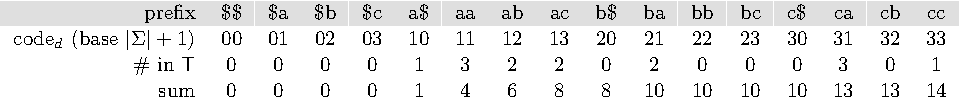
\includegraphics{kapitel/saca_algorithmen/bpr/algorithmus/beispiel/phase_1/step_02/bkt/image.pdf}}\par\medskip
        \resizebox{\textwidth}{!}{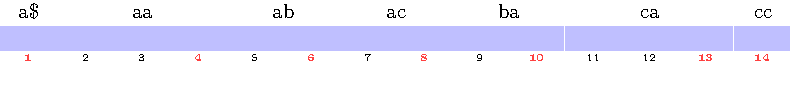
\includegraphics{kapitel/saca_algorithmen/bpr/algorithmus/beispiel/phase_1/step_02/buckets/image.pdf}}
    \end{minipage}}
    \caption[\bpr: Phase 1, Schritt 2]{\bpr: Phase 1, Schritt 2. Oben: Größen und Positionen der Buckets. Unten: Leere Buckets im Suffix-Array.}
    \label{bpr:p1s2}
\end{figure}
Im zweiten Schritt wird der Bucketsort Algorithmus (\cref{section:bucketsort}) durchgeführt, um eine Vorsortierung für das Suffix-Array zu erlangen. Die Tiefe, die für Bucketsort als Parameter verwendet wird, leitet sich in festgelegten Stufen aus der Größe des Alphabets ab und beträgt auch für große Alphabete mindestens 3. In diesem Beispiel wird aus Gründen der Übersichtlichkeit nur eine Tiefe von 2 verwendet.\par
\begin{figure}[H]
    {\centering\begin{minipage}{\textwidth}
        {\large \textsc{Schritt 3}}\par\medskip
        \resizebox{\textwidth}{!}{
            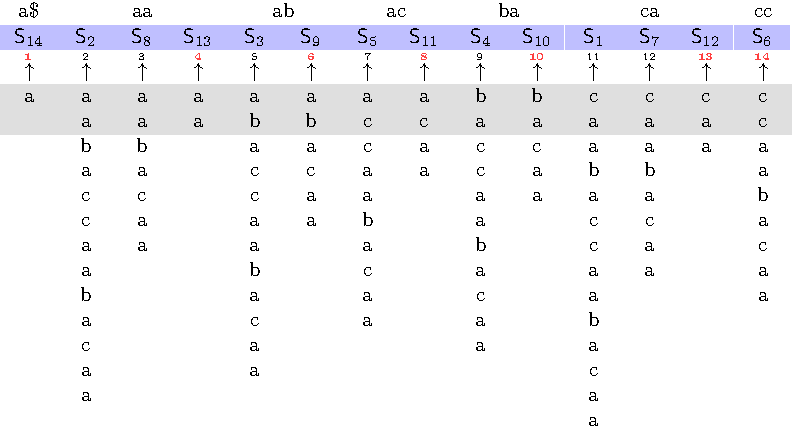
\includegraphics{kapitel/saca_algorithmen/bpr/algorithmus/beispiel/phase_1/step_03/buckets/image.pdf}
        }
        \resizebox{\textwidth}{!}{
            \includegraphics{kapitel/saca_algorithmen/bpr/algorithmus/beispiel/phase_1/step_03/bptr/image.pdf}
        }
    \end{minipage}}
    \caption[\bpr: Phase 1, Schritt 3]{\bpr: Phase 1, Schritt 3. Links: Befüllte Buckets im Suffix-Array. Rechts Initiales \bptr-Array.}
    \label{bpr:p1s3}
\end{figure}
Zu Beginn des dritten Schrittes sind die rechten Grenzen der Buckets bereits bekannt (siehe \cref{bpr:p1s2}, rot markiert und \cref{bpr:p1s3}, oben) und die Suffixe in die entsprechenden Buckets einsortiert. Daraus wird im Anschluss das Bucket-Pointer Array (\cref{bpr:p1s3}, unten) berechnet, in dem für jeden Suffix gespeichert ist, in welchem Bucket sich dieser in der aktuellen Sortierung befindet. Die Buckets werden dabei über ihre rechte inklusive Grenze identifiziert.\par
Sobald die Bucket-Pointer bestimmt sind, ist ein Zustand erreicht, von dem aus im Anschluss in der zweiten Phase alle Buckets Schritt für Schritt verfeinert werden können. Diese Verfeinerung erfolgt iterativ über die Buckets und rekursiv innerhalb der Buckets. Die Reihenfolge, in der die nach Phase 1 entstandenen Buckets sortiert werden, ist im Grundalgorithmus für die Korrektheit irrelevant. Unter Verwendung der Copy-Technik lässt sich der Rechenaufwand aber durch eine geschickte Wahl der Reihenfolge verringern.\par
\begin{figure}[H]
    {\centering\begin{minipage}{\textwidth}
        {\large \textsc{Schritt 1 (vorher)}} \hfill {\Large \textsc{Phase 2}}\par\medskip
        \resizebox{\textwidth}{!}{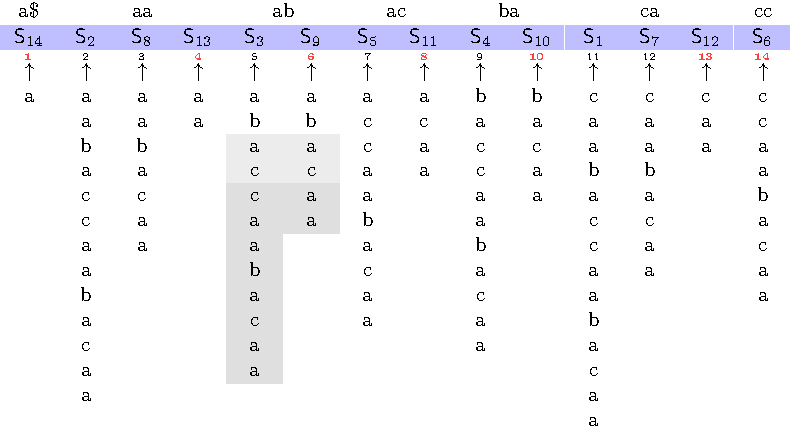
\includegraphics{kapitel/saca_algorithmen/bpr/algorithmus/beispiel/phase_2/step_01/buckets_before/image.pdf}}
        \resizebox{\textwidth}{!}{\includegraphics{kapitel/saca_algorithmen/bpr/algorithmus/beispiel/phase_2/step_01/bptr_before/image.pdf}}
    \end{minipage}}
    \caption[\bpr: Phase 2, Schritt 1 (vorher)]{\bpr: Phase 2, Schritt 1. \sa und \bptr vor dem Sortierschritt.}
    \label{bpr:p2s1:1}
\end{figure}
\begin{figure}[H]
    {\centering\begin{minipage}{\textwidth}
        {\large \textsc{Schritt 1 (nachher)}} \hfill {\Large \textsc{Phase 2}}\par\medskip
        \resizebox{\textwidth}{!}{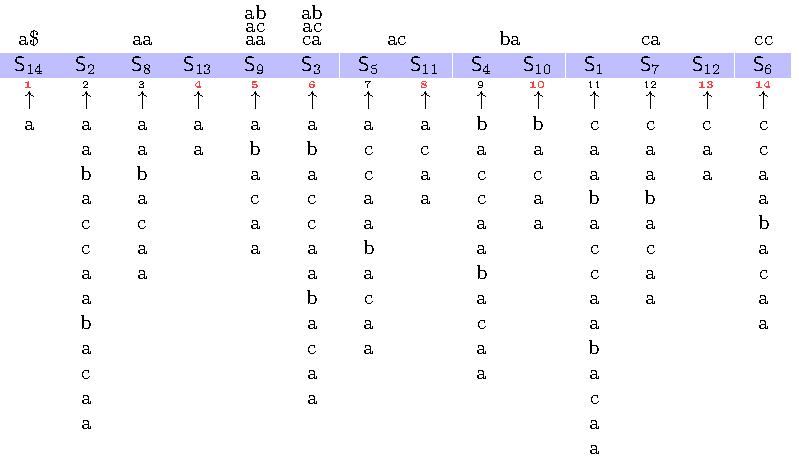
\includegraphics{kapitel/saca_algorithmen/bpr/algorithmus/beispiel/phase_2/step_01/buckets_after/image.pdf}}
        \resizebox{\textwidth}{!}{\includegraphics{kapitel/saca_algorithmen/bpr/algorithmus/beispiel/phase_2/step_01/bptr_after/image.pdf}}
    \end{minipage}}
    \caption[\bpr: Phase 2, Schritt 1 (nachher)]{\bpr: Phase 2, Schritt 1. \sa und \bptr nach dem Sortierschritt.}
    \label{bpr:p2s1:2}
\end{figure}
Die Verfeinerung erfolgt innerhalb eines Buckets Schrittweise mit einer Schrittgröße, die der zuvor gewählten Tiefe von Bucketsort entspricht. In diesem Beispiel wird zuerst der Bucket \bucket{ab} verfeinert. Aus der Bucket-Pointer Tabelle lässt sich nach einem Rekursionsschritt ablesen, dass die beiden darin enthaltenen Suffixe in ihrer Reihenfolge vertauscht werden müssen. Danach ist der Bucket fertig sortiert und die Bucket-Pointer werden an die neue Sortierung angepasst.\par
\begin{figure}[H]
    {\centering\begin{minipage}{\textwidth}
        {\large \textsc{Schritt 2 (vorher)}}\par\medskip
        \resizebox{\textwidth}{!}{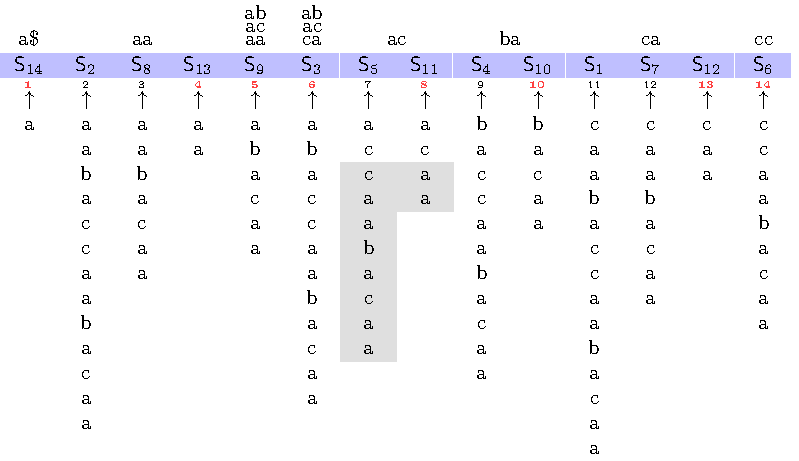
\includegraphics{kapitel/saca_algorithmen/bpr/algorithmus/beispiel/phase_2/step_02/buckets_before/image.pdf}}
        \resizebox{\textwidth}{!}{\includegraphics{kapitel/saca_algorithmen/bpr/algorithmus/beispiel/phase_2/step_02/bptr_before/image.pdf}}
    \end{minipage}}
    \caption[\bpr: Phase 2, Schritt 2 (vorher)]{\bpr: Phase 2, Schritt 2. \sa und \bptr vor dem Sortierschritt.}
    \label{bpr:p2s2:1}
\end{figure}
\begin{figure}[H]
    {\centering\begin{minipage}{\textwidth}
        {\large \textsc{Schritt 2 (nachher)}}\par\medskip
        \resizebox{\textwidth}{!}{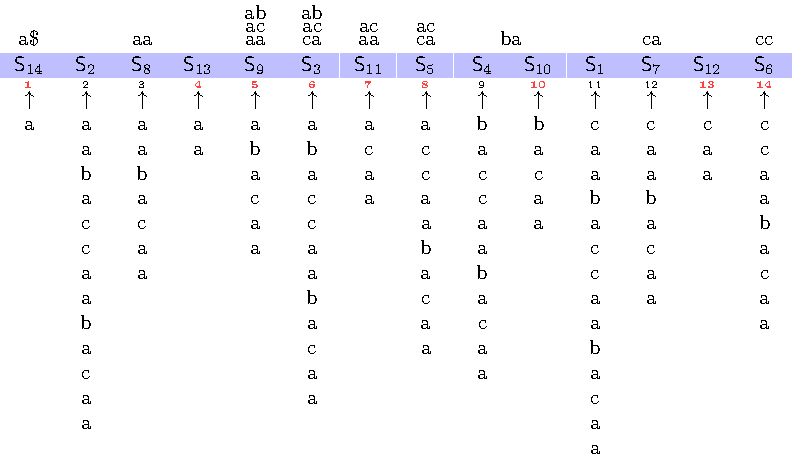
\includegraphics{kapitel/saca_algorithmen/bpr/algorithmus/beispiel/phase_2/step_02/buckets_after/image.pdf}}
        \resizebox{\textwidth}{!}{\includegraphics{kapitel/saca_algorithmen/bpr/algorithmus/beispiel/phase_2/step_02/bptr_after/image.pdf}}
    \end{minipage}}
    \caption[\bpr: Phase 2, Schritt 2 (nachher)]{\bpr: Phase 2, Schritt 2. \sa und \bptr nach dem Sortierschritt.}
    \label{bpr:p2s2:2}
\end{figure}
Anschließend wird der Bucket \bucket{ac} sortiert (\cref{bpr:p2s2:1,bpr:p2s2:2}), dessen Suffixe sich bereits nach einem gemeinsamen Präfix der Länge 2 unterscheiden. Aus der Bucket-Pointer Tabelle kann damit direkt abgelesen werden, in welchen Buckets sich die korrespondierenden Suffixe befinden, woraus dann die Reihenfolge abgeleitet wird. Das Vertauschen von \(\suffix{5}\) und \(\suffix{11}\) führt zur richtigen Reihenfolge.\par
Die darauf folgende Sortierung des Buckets \bucket{ba} erfolgt analog (\cref{bpr:p2s3:1,bpr:p2s3:2}).
\begin{figure}[H]
    {\centering\begin{minipage}{\textwidth}
        {\large \textsc{Schritt 3 (vorher)}}\par\medskip
        \resizebox{\textwidth}{!}{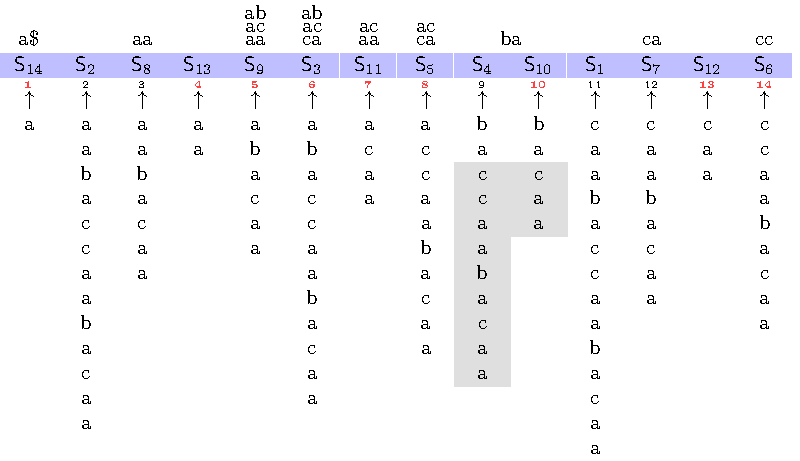
\includegraphics{kapitel/saca_algorithmen/bpr/algorithmus/beispiel/phase_2/step_03/buckets_before/image.pdf}}
        \resizebox{\textwidth}{!}{\includegraphics{kapitel/saca_algorithmen/bpr/algorithmus/beispiel/phase_2/step_03/bptr_before/image.pdf}}
    \end{minipage}}
    \caption[\bpr: Phase 2, Schritt 3 (vorher)]{\bpr: Phase 2, Schritt 3. \sa und \bptr vor dem Sortierschritt.}
    \label{bpr:p2s3:1}
\end{figure}
\begin{figure}[H]
    {\centering\begin{minipage}{\textwidth}
        {\large \textsc{Schritt 3 (nachher)}}\par\medskip
        \resizebox{\textwidth}{!}{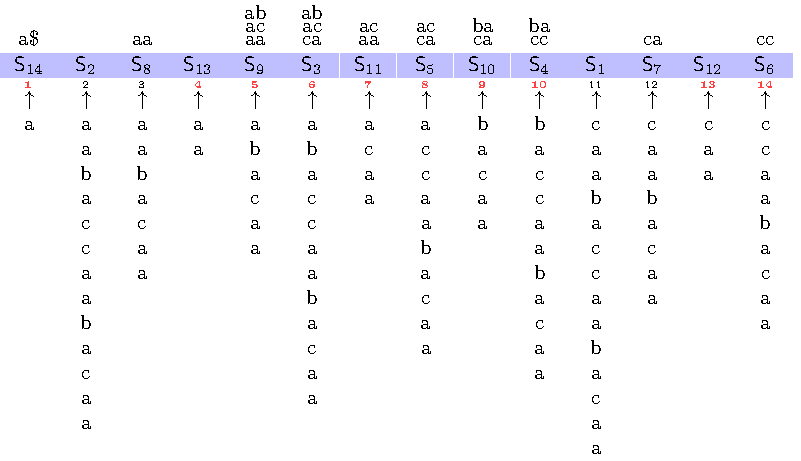
\includegraphics{kapitel/saca_algorithmen/bpr/algorithmus/beispiel/phase_2/step_03/buckets_after/image.pdf}}
        \resizebox{\textwidth}{!}{\includegraphics{kapitel/saca_algorithmen/bpr/algorithmus/beispiel/phase_2/step_03/bptr_after/image.pdf}}
    \end{minipage}}
    \caption[\bpr: Phase 2, Schritt 3 (nachher)]{\bpr: Phase 2, Schritt 3. \sa und \bptr nach dem Sortierschritt.}
    \label{bpr:p2s3:2}
\end{figure}
Zuletzt werden in den Schritten 4 und 5 (\cref{bpr:p2s4:1,bpr:p2s4:2} sowie \cref{bpr:p2s5:1,bpr:p2s5:2}) die Buckets \bucket{aa} und \bucket{ca} sortiert. Beide bestehen aus jeweils drei Suffixen, die sich alle bereits eindeutig anhand der Positionen in der nebenstehenden Tabelle in Buckets der Größe 1 einsortieren lassen. Nach Schritt 5 existieren schließlich nur noch Buckets der Größe 1 und das Suffix-Array ist damit fertig sortiert. An dieser Stelle verwirft der Algorithmus das Array \bptr und gibt \sa als Lösung aus.
\begin{figure}[H]
    {\centering\begin{minipage}{\textwidth}
        {\large \textsc{Schritt 4 (vorher)}}\par\medskip
        \resizebox{\textwidth}{!}{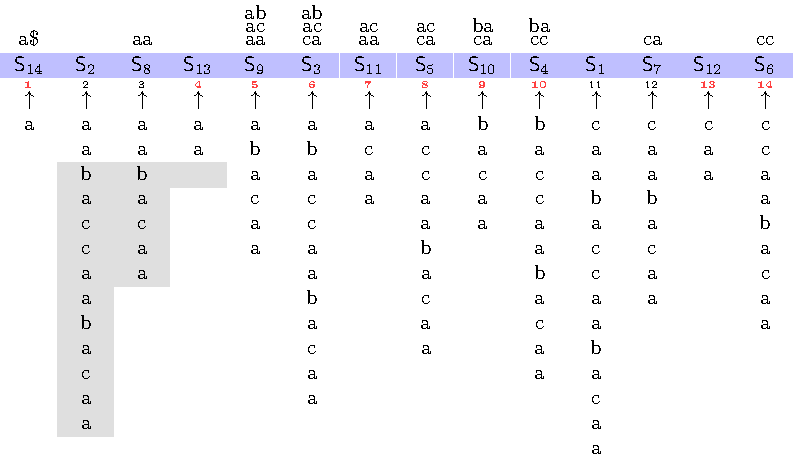
\includegraphics{kapitel/saca_algorithmen/bpr/algorithmus/beispiel/phase_2/step_04/buckets_before/image.pdf}}
        \resizebox{\textwidth}{!}{\includegraphics{kapitel/saca_algorithmen/bpr/algorithmus/beispiel/phase_2/step_04/bptr_before/image.pdf}}
    \end{minipage}}
    \caption[\bpr: Phase 2, Schritt 4 (vorher)]{\bpr: Phase 2, Schritt 4. \sa und \bptr vor dem Sortierschritt.}
    \label{bpr:p2s4:1}
\end{figure}
\begin{figure}[H]
    {\centering\begin{minipage}{\textwidth}
        {\large \textsc{Schritt 4 (nachher)}}\par\medskip
        \resizebox{\textwidth}{!}{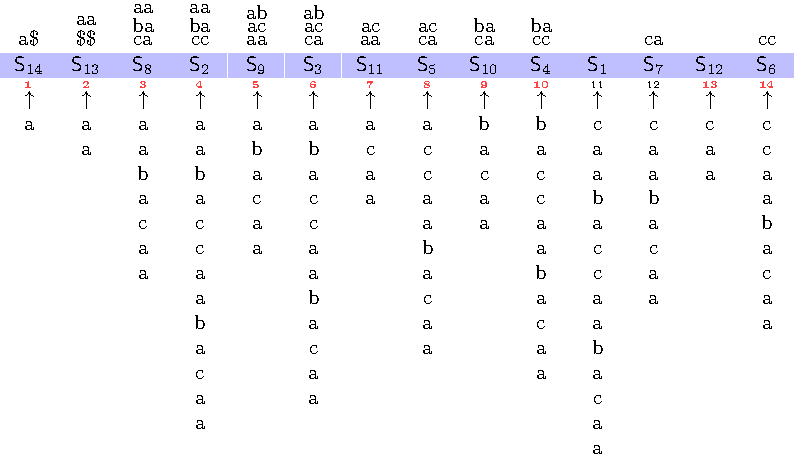
\includegraphics{kapitel/saca_algorithmen/bpr/algorithmus/beispiel/phase_2/step_04/buckets_after/image.pdf}}
        \resizebox{\textwidth}{!}{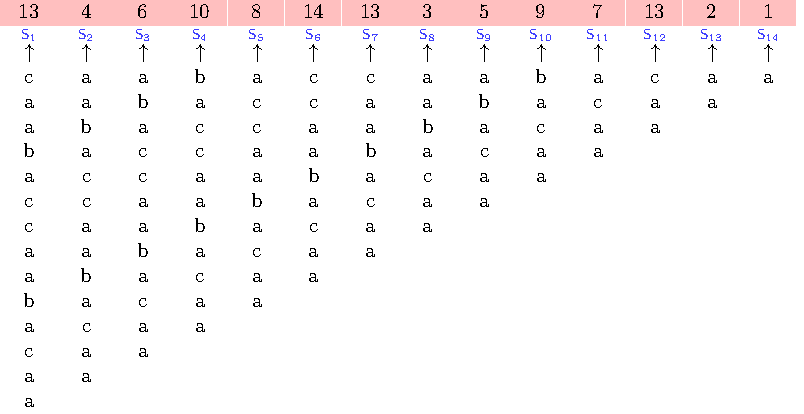
\includegraphics{kapitel/saca_algorithmen/bpr/algorithmus/beispiel/phase_2/step_04/bptr_after/image.pdf}}
    \end{minipage}}
    \caption[\bpr: Phase 2, Schritt 4]{\bpr: Phase 2, Schritt 4. \sa und \bptr nach dem Sortierschritt.}
    \label{bpr:p2s4:2}
\end{figure}
\begin{figure}[H]
    {\centering\begin{minipage}{\textwidth}
        {\large \textsc{Schritt 5 (vorher)}}\par\medskip
        \resizebox{\textwidth}{!}{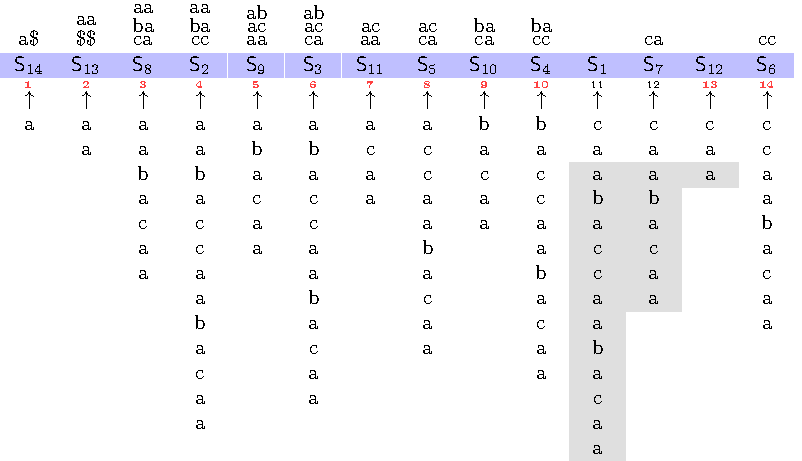
\includegraphics{kapitel/saca_algorithmen/bpr/algorithmus/beispiel/phase_2/step_05/buckets_before/image.pdf}}
        \resizebox{\textwidth}{!}{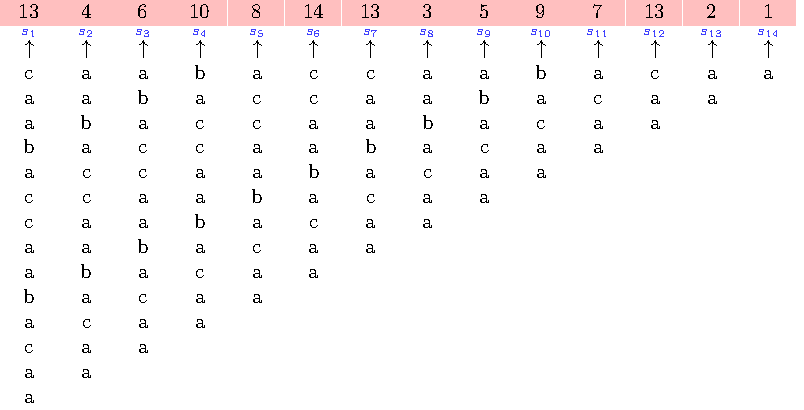
\includegraphics{kapitel/saca_algorithmen/bpr/algorithmus/beispiel/phase_2/step_05/bptr_before/image.pdf}}
    \end{minipage}}
    \caption[\bpr: Phase 2, Schritt 5 (vorher)]{\bpr: Phase 2, Schritt 5. \sa und \bptr vor dem Sortierschritt.}
    \label{bpr:p2s5:1}
\end{figure}
\begin{figure}[H]
    {\centering\begin{minipage}{\textwidth}
        {\large \textsc{Schritt 5 (nachher)}}\par\medskip
        \resizebox{\textwidth}{!}{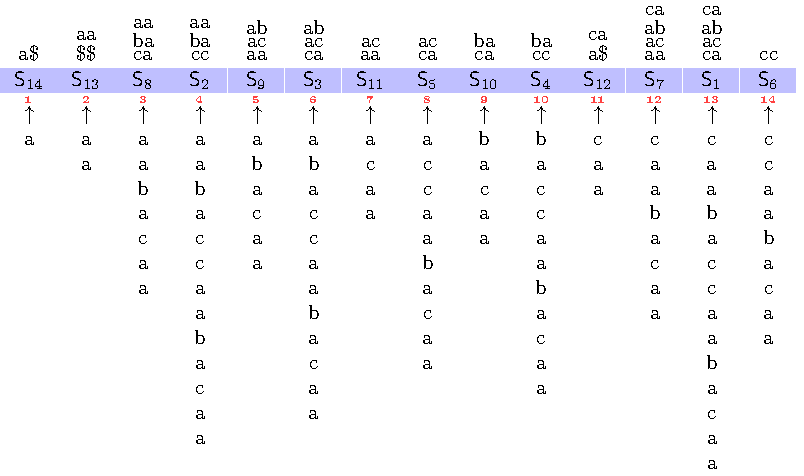
\includegraphics{kapitel/saca_algorithmen/bpr/algorithmus/beispiel/phase_2/step_05/buckets_after/image.pdf}}
        \resizebox{\textwidth}{!}{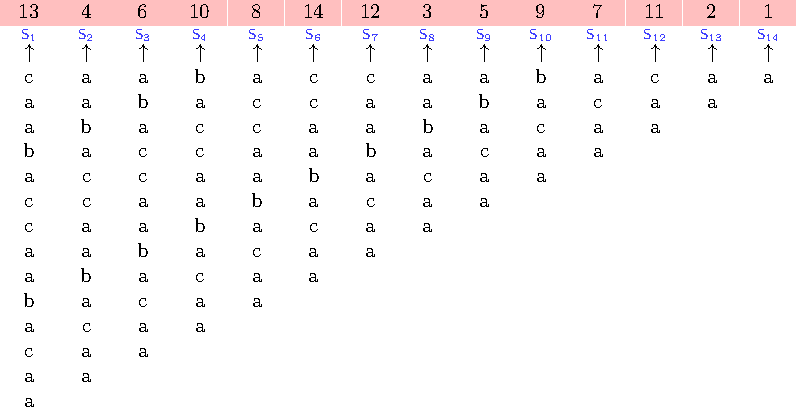
\includegraphics{kapitel/saca_algorithmen/bpr/algorithmus/beispiel/phase_2/step_05/bptr_after/image.pdf}}
    \end{minipage}}
    \caption[\bpr: Phase 2, Schritt 5 (nachher)]{\bpr: Phase 2, Schritt 5. \sa und \bptr nach dem Sortierschritt.}
    \label{bpr:p2s5:2}
\end{figure}
